\documentclass[11pt]{article}
\usepackage{amsmath,amssymb,graphicx}
\usepackage{../setspace}
\addtolength{\textwidth}{1.5in}
\addtolength{\hoffset}{-1in}
\addtolength{\textheight}{1.5in}
\addtolength{\voffset}{-1in}

\title{STAT3401: Lab exercises concerning principal components}
\author{Paul Hewson}
\date{11th January 2007}
\usepackage{/usr/share/R/share/texmf/Sweave}
\begin{document}
\setlength{\parindent}{0pt}
\setlength{\parskip}{12pt}
\sffamily
\maketitle




Do note that the Heptathalon data, and code for two functions are available in the portal!

First, the data needs to be removed from the portal, and loaded into \textbf{R}.   Then, as explained in the lecture, some rescaling is necessary:


\begin{Schunk}
\begin{Sinput}
> hept.df <- read.csv("Heptathalon.csv", row.names = 1)
> hept.df$X100mHurdles.S. <- hept.df$X100mHurdles.S. * -1
> hept.df$X200m.sec. <- hept.df$X200m.sec. * -1
> hept.df$r800m.s. <- hept.df$r800m.s. * -1
\end{Sinput}
\end{Schunk}

You may like to consider whether this particular rescaling is a good one.   Perhaps it would have been better to take reciprocals?


\section{A principal components analysis}

Essentially, all we need to carry out a principal component analysis are the eigenvalues and eigenvectors of the covariance or correlation matrix.   This is as simple as:

\begin{Schunk}
\begin{Sinput}
> hept.cormat <- cor(hept.df[,-1])
> hept.covmat <- cov(hept.df[,-1])
> hep1.ev <- eigen(hept.cormat)
> hep1.ev
> hep2.ev <- eigen(hept.covmat)
> hep2.ev
\end{Sinput}
\end{Schunk}

And a scree plot can be quite easily obtained using \verb+plot(hep1.ev$values, type = "b")+


\section{Using the in-built functions}

In practice, we will use the inbuilt functions.   There is an older function, \texttt{princomp()}, which is retained partly for compatibility with S-Plus and partly because it allows us to provide a covariance matrix to the function (such as a robust estimate rather than the usual estimator).   The advantage of using the inbuilt functions are that the objects created have various methods associated.

\begin{Schunk}
\begin{Sinput}
> hept.princomp <- princomp(hept.df[,-1], scale = TRUE)
> summary(hept.princomp)
> plot(hept.princomp) ## produces scree plot
> biplot(hept.princomp) ## produces biplot
> loadings(hept.princomp) ## pretty printed 
> predict(hept.princomp) ## scores
> par(mfrow = c(3,3))
> apply(predict(hept.princomp), 2, qqnorm)
\end{Sinput}
\end{Schunk}

The latter two lines are a reminder that if the original data were multivariate normal, then all the infinite linear combinations (including the principal components) will be univariate normal.

\begin{itemize}
\item Why did we add the instruction \verb+scale = TRUE+ in the call to \verb+princomp()+.   What is the analagous instruction to the command \verb+prcomp()+
\item How many components do you wish to retain in the heptathalon analysis?
\item Can you interpret the principal components (by altering the arguments to \verb+choices+ you can examine different variables, e.g.  \verb+biplot(hept.princomp,choices = c(1,3))+)?
\item Do the principal component scores suggest a different method for awarding medals (details on the actual winner can be found on the web)?
\end{itemize}


\begin{itemize}
\item Before moving on, it is a very good idea to conduct a principal component analysis of the US Arrests data: contrast the scree plot from an analysis based on the covariance matrix and an analysis based on the correlation matrix?   What information does the former analysis give you?
\end{itemize}


\section{Using \texttt{prcomp()}}

\texttt{prcomp()} uses the original data, and do note that it returns the square roots of the eigenvalues (in principle at least).   We use this routine to examine the turtles data:

\begin{Schunk}
\begin{Sinput}
> library(Flury)
> data(turtles)
\end{Sinput}
\end{Schunk}

The helpfile gives you one suggestion for eda.   We follow Flury (1997) below, and consider only the males.   We take natural logarithms and multiply the values by 10.

\begin{Schunk}
\begin{Sinput}
> data(turtles)
>   turtles.m <- subset(turtles, turtles$Gender == "Male")
>   turtles.m <- 10 * log(turtles.m[,-1])
>   turtles.m.prcomp <- prcomp(turtles.m)
>   summary(turtles.m.prcomp)
> plot(turtles.m.prcomp)
> turtles.m.prcomp$sdev^2 ## extract eigenvalues
> par(xpd = NA)
> biplot(turtles.m.prcomp)
\end{Sinput}
\end{Schunk}

\begin{itemize}
\item How many principal components do you need to retain here?
\item How do you interpret the principal components?
\end{itemize}


\section{Aside: the value of reducing dimensions}

Here's a lot of code we've seen before, it produces a three cluster solution from five variables collected on mammalian milk.   We tried plotting the cluster solutions against the original data - but perhaps we don't need a five dimensional representation.   The last five lines try plotting the cluster solution against the first two principal components.   Some of the inbuilt visulisation functions in the \texttt{cluster} library do this for you!

\begin{Schunk}
\begin{Sinput}
> library(cluster)
> library(flexclust)
> data(milk)
> milk.dist <- dist(milk)
> milk.hclust <- hclust(milk.dist)
> plot(milk.hclust)
> milk.cut <- cutree(milk.hclust, 3)
> z <- predict(prcomp(milk, scale = TRUE)) ##a
> plot(z, col = milk.cut, pch = milk.cut, main = "a")
> ## run the command windows() to compare these side by side
> z <- predict(prcomp(milk, scale = FALSE)) ##b
> plot(z, col = milk.cut, pch = milk.cut, main = "b")
\end{Sinput}
\end{Schunk}

\begin{itemize}
\item What's the difference between graph $a$ and $b$.
\end{itemize}

\section{Further routines for considering the number of dimensions needed}

(R code for the two functions, \texttt{Horn()} and \texttt{stickometer()} is available from the portal - improvements and suggestions are most welcome)


Here we consider Horn's method for simulating from the sample covariance matrix:

\begin{Schunk}
\begin{Sinput}
> require(MASS)
> Horn <- function(data, reps){
+   p <- dim(data)[2]
+   n <- dim(data)[1]
+   Varmat <- matrix(0,p,p)
+   Mean <- mean(data)
+   diag(Varmat) <- diag(var(data))
+     Evals <- princomp(data, cor = TRUE)$sdev^2
+     idx <- barplot(Evals, names.arg = paste("PC", c(1:7)), 
+     xlab = "Component", ylab = "Proportion of trace", 
+     main = "Proportion of trace explained")
+       results <- matrix(0,reps,p)
+       for (i in 1:reps){
+       SimData <- mvrnorm(n, Mean, Varmat)
+       ExpEvalsH <- princomp(SimData, cor = TRUE)$sdev^2
+       results[i,] <- ExpEvalsH
+       lines(idx, ExpEvalsH, type = "b", pch = 16)
+       }
+     lines(idx, apply(results, 2, mean), type = "b", col = "red")
+   legend("topright", lty = 1, pch = 16, legend = "Expected values")
+   Results <- data.frame(Evals = Evals, ExpEvalsH = ExpEvalsH)
+ }
\end{Sinput}
\end{Schunk}


Having entered this function (it is available in the portal), it can be used on the heptathalon data simply by entering:

\begin{Schunk}
\begin{Sinput}
> Horn(hept.df[-1], 10)
\end{Sinput}
\end{Schunk}
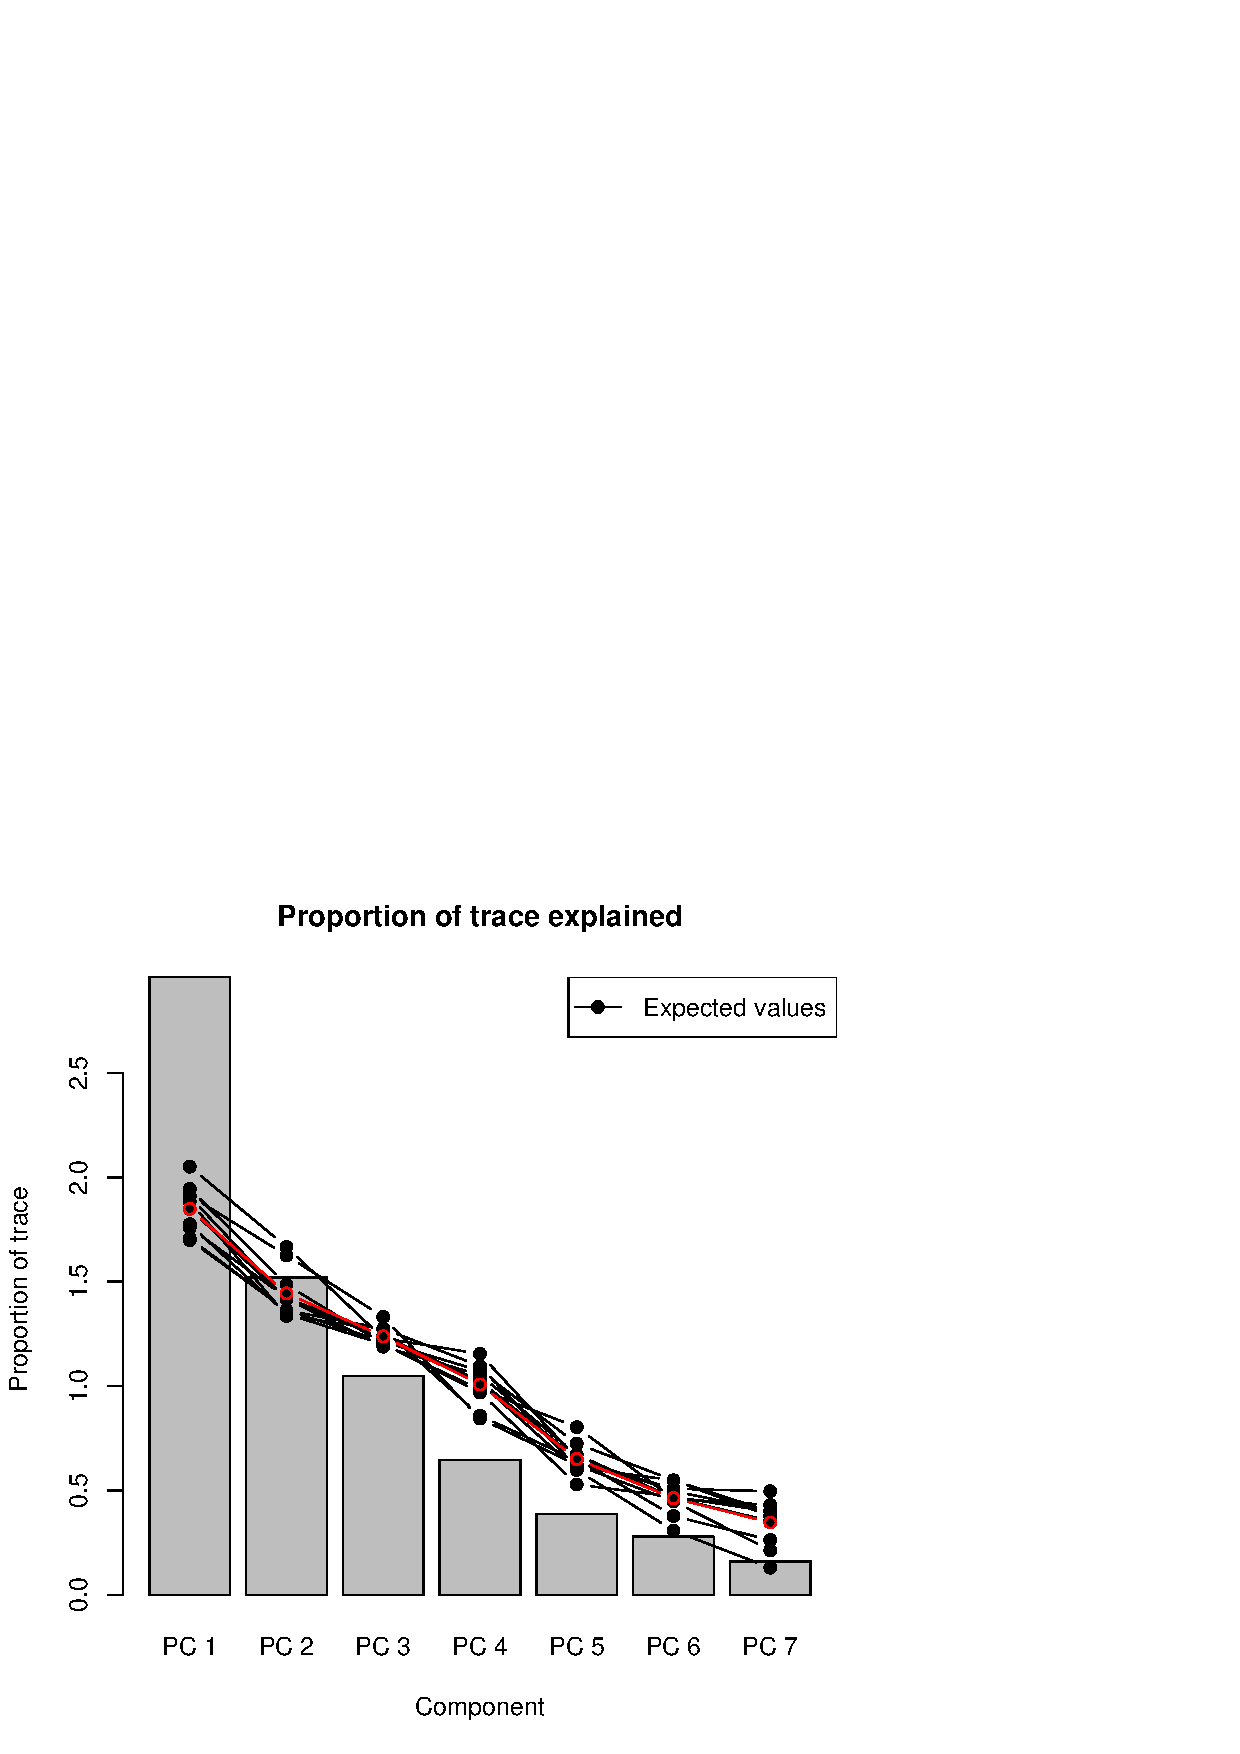
\includegraphics{STAT3401Week5PCAlab-hornhept}
to get ten replicates.  You may wish to consider more than 10.


In a similar way, we can get Joliffe's stick estimates as follows:

\begin{Schunk}
\begin{Sinput}
>  stickometer <- function(p){
+   vec <- 1 / (1:p)
+   stick <- vector("numeric", p) 
+   stick[1] <- sum(vec)
+      for (i in 2:p){
+      stick[i] <- sum(vec[-(1:(i-1))])}
+   stick <- 1/p * stick
+   names(stick) <- paste("Comp.", c(1:p), sep = "")
+   return(stick)
+ }
\end{Sinput}
\end{Schunk}

And so, for the heptathalon data (we created the \texttt{hept.princomp} object earlier), we can create a barplot of the proportion of variance explained and superimpose a line from the expected values as follows:

\begin{Schunk}
\begin{Sinput}
>  stick <- stickometer(7)
>  proptrace <- hept.princomp$sdev^2 / sum(hept.princomp$sdev^2)
>  stick ## checking the values
>  proptrace ## checking the values
>  idx <- barplot(proptrace, names.arg = paste("PC", c(1:7)), 
+  xlab = "Component", ylab = "Proportion of trace", 
+  main = "Proportion of trace explained")
>  lines(idx, stick, type = "b", pch = 16)
>  legend("topright", lty = 1, pch = 16, legend = "Expected values")
\end{Sinput}
\end{Schunk}
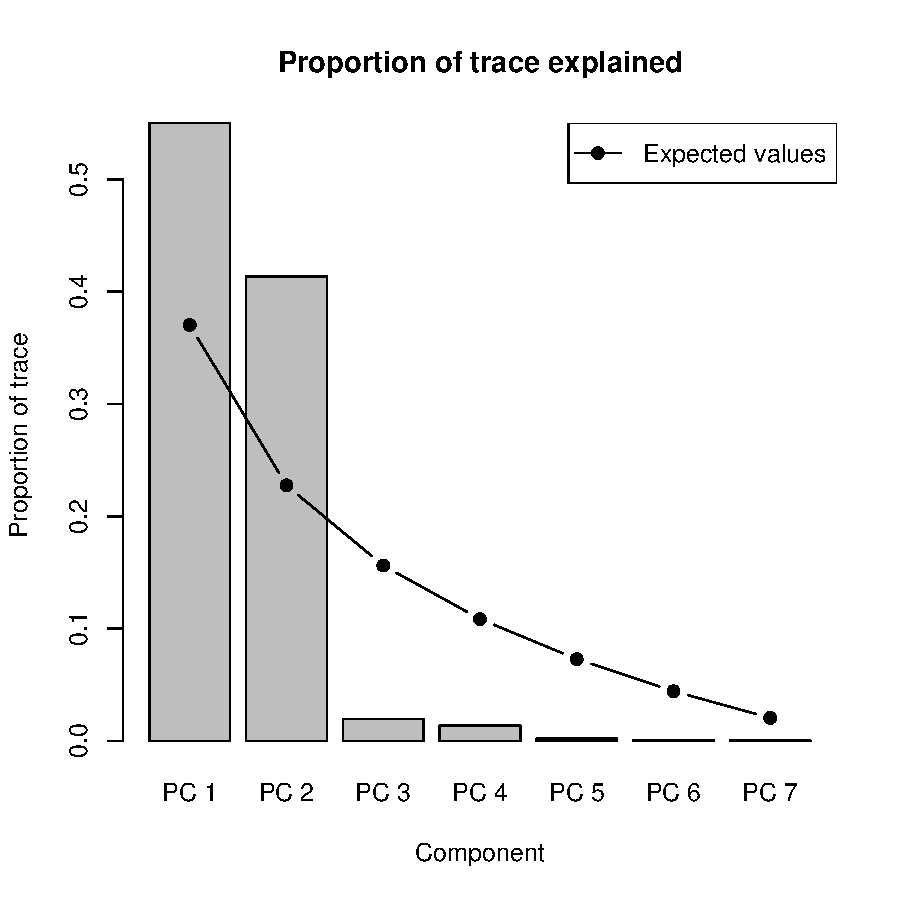
\includegraphics{STAT3401Week5PCAlab-stickhept}

It would be nice to see this laid out properly!


\begin{itemize}
\item Does either method alter your recommendation as to how many principal components should be retained?
\item What alterations need to be be made to the line:
\begin{verbatim}
proptrace <- hept.princomp$sdev^2 / sum(hept.princomp$sdev^2)
\end{verbatim}
in order to work with \texttt{prcomp()} objects?
\end{itemize}


\section{Examining the Mahalanobis distance}

The following function will partition the Mahalanobis distance between the retained and non-retained components:

\begin{Schunk}
\begin{Sinput}
> princomp2dist <- function(obj.princomp, retain){
+  scores <- t(t(obj.princomp$scores^2) / obj.princomp$sdev)
+  dtot <- apply(scores, 1, sum)
+  d1 <- apply(scores[,c(1:retain)], 1, sum)
+  d2 <- apply(scores[,-c(1:retain)], 1, sum)
+  dists <- data.frame(dtot = dtot, d1 = d1, d2 = d2)
+  return(dists)
+ }
\end{Sinput}
\end{Schunk}


So for example, if we wanted to retain three components from the heptathalon data we could use the following:

\begin{Schunk}
\begin{Sinput}
> hept.princomp <- princomp(hept.df[-1], scores = TRUE, scale = TRUE)
> ## form a princomp object
> hept.m <- princomp2dist(hept.princomp, 3)
\end{Sinput}
\end{Schunk}


All that remains to be done is to plot the retained distances as a suitable qq plot.   One could also consider a scatter plot of retained versus non-retained distances to see if there are any individuals who are not well explained by the 3 dimensional representation using something like \verb+plot(hept.m$d1, hept.m$d2)+


\end{document}


